\chapter{Kiến trúc ứng dụng iOS}
\label{Kiến trúc hệ điều hành iOS}

\begin{flushleft}
\hspace{1em}\parbox{\dimexpr\textwidth-2em}{

\vspace{0.5em}Kiến trúc hệ điều hành iOS được xây dựng theo kiến trúc phân lớp, hệ điều hành iOS cung cấp một nền tảng mạnh mẽ và linh hoạt cho các thiết bị di động của Apple. Gồm bốn lớp chính, kiến trúc này giúp tổ chức hệ thống một cách rõ ràng và hiệu quả.

\vspace{0.5em}Cung cấp giao diện người dùng và xử lý các tương tác cảm ứng, lớp \textbf{Cocoa Touch} là lớp cao nhất trong kiến trúc. Sử dụng các framework như \texttt{UIKit}, \texttt{MapKit}, và \texttt{MessageUI}, lớp này cho phép nhà phát triển tạo ra những ứng dụng thân thiện và trực quan.

\vspace{0.5em}Hỗ trợ các chức năng đồ họa, âm thanh và video, lớp \textbf{Media} đóng vai trò quan trọng trong việc xử lý nội dung đa phương tiện. Thông qua các framework như \texttt{Core Graphics}, \texttt{AVFoundation}, và \texttt{Core Animation}, lớp này tạo nên trải nghiệm hình ảnh sống động và chân thực.

\vspace{0.5em}Cung cấp các dịch vụ nền tảng như quản lý dữ liệu, mạng và vị trí, lớp \textbf{Core Services} đảm bảo hoạt động ổn định cho ứng dụng. Các thành phần như \texttt{Core Data}, \texttt{Core Foundation} và \texttt{CFNetwork} là những công cụ thiết yếu cho lập trình viên.

\vspace{0.5em}Làm nền tảng cho toàn bộ hệ thống, lớp \textbf{Core OS} chịu trách nhiệm giao tiếp với phần cứng và điều phối tài nguyên hệ thống. Với nhân Darwin và các dịch vụ hệ thống bảo mật, lớp này giúp iOS vận hành ổn định, an toàn và hiệu quả.

\vspace{0.5em}Nhờ sự phân chia rõ ràng và logic giữa các lớp, kiến trúc iOS hỗ trợ phát triển ứng dụng một cách tối ưu, đồng thời đảm bảo hiệu suất và tính bảo mật cao trên các thiết bị di động.
}
\end{flushleft}
\label{chap:IOS}


\section{Nền tảng iOS và các thành phần cơ bản}
\hspace*{0.8cm}iOS là hệ điều hành di động do Apple phát triển, được sử dụng chủ yếu trên các thiết bị như iPhone, iPad và iPod Touch. Với kiến trúc nhiều tầng cùng hệ sinh thái phong phú, iOS cung cấp môi trường ổn định, bảo mật và hiệu năng cao cho việc phát triển ứng dụng di động. Để xây dựng một ứng dụng iOS hiệu quả, lập trình viên cần nắm vững các thành phần cơ bản như vòng đời ứng dụng, delegate, giao diện người dùng, cũng như các mô hình kiến trúc phổ biến. Phần này sẽ trình bày tổng quan về các yếu tố cốt lõi tạo nên nền tảng iOS và vai trò của chúng trong quy trình phát triển ứng dụng.
    \subsection{Kiến trúc tầng của iOS}
        \begin{flushleft}
            \begin{figure}[H] % hoặc [h], [t], [b] tùy vị trí
                \centering
                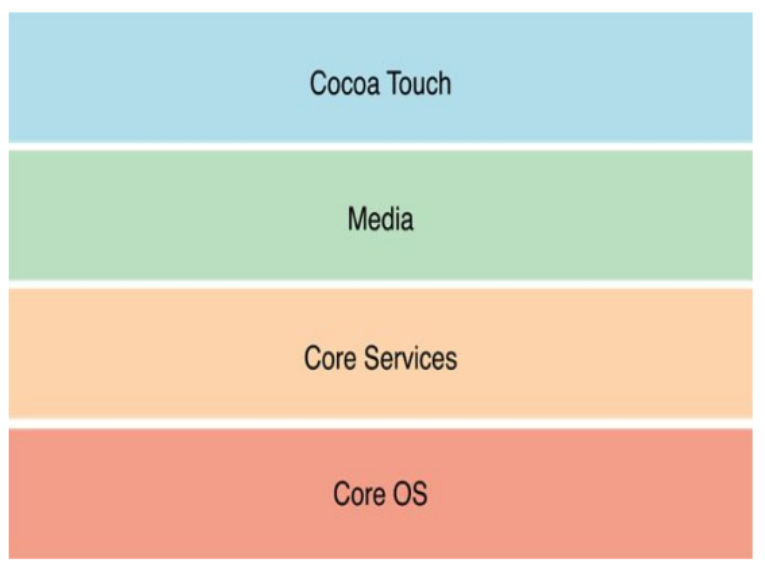
\includegraphics[width=0.8\textwidth]{images/kientrucios.png}
                \caption{Kiến trúc phân tầng IOS\cite{kientrucios}.}
                \label{fig:kientrucios}
            \end{figure}

            \hspace*{0.8cm}Hệ điều hành iOS được tổ chức theo kiến trúc nhiều tầng, trong đó mỗi tầng đảm nhận một vai trò cụ thể và cung cấp các framework cũng như dịch vụ khác nhau. Ở tầng cao nhất, \textbf{Cocoa Touch} cung cấp các framework cốt lõi dành cho việc xây dựng giao diện người dùng, đáng chú ý là \textit{UIKit} và \textit{SwiftUI}. Các công nghệ đồ họa, âm thanh và video như \textit{Core Graphics}, \textit{Core Animation}, và \textit{AVFoundation} được tập trung tại tầng \textbf{Media}, giúp xử lý các chức năng đa phương tiện. Bên dưới đó, tầng \textbf{Core Services} cung cấp các dịch vụ nền tảng cần thiết như \textit{Core Data} để quản lý dữ liệu, \textit{Core Location} để định vị, và \textit{Foundation framework} cho các chức năng cơ bản. Cuối cùng, tầng \textbf{Core OS} đóng vai trò là nền tảng thấp nhất của hệ điều hành, nơi tích hợp kernel, hệ thống tệp, các cơ chế bảo mật và các dịch vụ hệ thống cấp thấp.

       
        \end{flushleft}
   \subsection{ Vòng đời ứng dụng IOS}	
        \begin{flushleft}
            \hspace*{0.8cm}Khi người dùng khởi động điện thoại, chỉ có các thành phần của hệ điều hành (\textit{Operating System}) được phép hoạt động, trong khi các ứng dụng của người dùng chưa được kích hoạt. Các ứng dụng, bao gồm cả ứng dụng của bạn, sẽ chỉ bắt đầu thực thi khi người dùng nhấn vào biểu tượng ứng dụng trên màn hình chính. Chính lúc đó, \textbf{Springboard} – trình quản lý giao diện màn hình chính của iOS – sẽ chịu trách nhiệm kích hoạt ứng dụng. Ứng dụng cùng với các thư viện liên quan sẽ được tải vào bộ nhớ và bắt đầu khởi chạy, trong khi đó \textbf{Springboard} sẽ hiển thị màn hình khởi động (launch screen) để tạo cảm giác phản hồi tức thì cho người dùng. Sau khi quá trình tải hoàn tất, ứng dụng sẽ bắt đầu thực thi, và \texttt{AppDelegate} – đối tượng chịu trách nhiệm quản lý vòng đời của ứng dụng 
            – sẽ nhận được các thông báo tương ứng từ hệ thống.
            Trong quá trình hoạt động, ứng dụng iOS luôn ở một trong các trạng thái xác định: \textbf{Not Running}, \textbf{Inactive}, \textbf{Active}, \textbf{Background}, hoặc \textbf{Suspended}. Những trạng thái này phản ánh tình huống hiện tại của ứng dụng đối với hệ điều hành, và tại bất kỳ thời điểm nào, ứng dụng của bạn đều sẽ nằm trong một trong các trạng thái đó. Việc hiểu rõ và xử lý đúng các trạng thái này là yếu tố then chốt để đảm bảo ứng dụng vận hành hiệu quả, tiết kiệm tài nguyên và mang lại trải nghiệm người dùng mượt mà.
            
        \end{flushleft}
        \begin{figure}[H] % hoặc [h], [t], [b] tùy vị trí
            \centering
            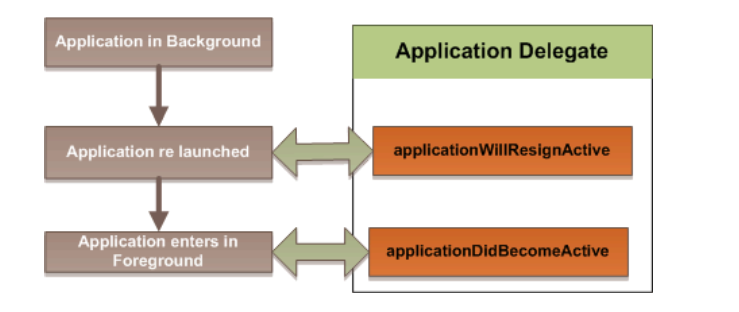
\includegraphics[width=0.8\textwidth]{images/vongdoiios.png}
             \caption{Vòng đời ứng dụng IOS\cite{life cycle-IOS}.} 
            \label{fig:vongdoiios}
        \end{figure}
         \begin{flushleft}
            \textbf{NotRunning:}Ứng dụng chưa được khởi chạy hoặc đã bị hệ thống chấm dứt.
            \textbf{Inactive:} Ứng dụng đang chạy ở foreground nhưng không nhận events (ví dụ: khi có cuộc gọi đến).\\
            \textbf{Active:} Trạng thái bình thường khi ứng dụng chạy ở foreground và đang xử lý events.\\
            \textbf{Background:} Ứng dụng không hiển thị nhưng vẫn chạy và thực thi mã.\\
            \textbf{Suspended:} Ứng dụng ở background nhưng không chạy mã, có thể bị hệ thống chấm dứt để giải phóng tài nguyên.
         \end{flushleft}
         \subsection{App Delegate và Scene Delegate}
         \hspace*{0.8cm}Trong iOS, hai thành phần quan trọng đảm nhận việc quản lý vòng đời và giao diện của ứng dụng là \textbf{AppDelegate} và \textbf{SceneDelegate}. \textbf{AppDelegate}\cite{ App-Scene Delegate} chịu trách nhiệm xử lý các sự kiện cấp cao liên quan đến vòng đời tổng thể của ứng dụng, chẳng hạn như khi ứng dụng được khởi động, chuyển sang chế độ nền, hoặc bị chấm dứt. Bên cạnh đó, nó cũng đảm nhiệm các tác vụ cấu hình ban đầu như đăng ký notification, khởi tạo dịch vụ, và thiết lập dữ liệu dùng chung.
         Kể từ iOS 13, Apple giới thiệu khái niệm \textbf{Scene} để hỗ trợ việc chạy nhiều cửa sổ giao diện (\textit{multi-window}) trong cùng một ứng dụng, đặc biệt trên iPad. Chính vì thế, \textbf{SceneDelegate} ra đời nhằm tách riêng trách nhiệm quản lý giao diện người dùng (UI lifecycle) cho từng scene. \textbf{SceneDelegate} xử lý các sự kiện như scene được kết nối, hiển thị, vào nền hoặc bị hủy, từ đó cho phép quản lý độc lập từng cửa sổ ứng dụng.
         Sự phân tách giữa \texttt{AppDelegate} và \texttt{SceneDelegate} giúp ứng dụng có kiến trúc rõ ràng hơn, dễ dàng mở rộng cho các thiết bị hỗ trợ đa cửa sổ, đồng thời tuân thủ tốt hơn nguyên lý phân chia trách nhiệm trong lập trình.

         \subsection{Luồng làm việc của người dùng và Storyboards}

        \hspace*{0.8cm}Trong quá trình phát triển ứng dụng iOS, việc thiết kế luồng di chuyển của người dùng giữa các màn hình là một phần quan trọng nhằm đảm bảo trải nghiệm sử dụng mượt mà và trực quan. Để hỗ trợ việc này, Apple cung cấp công cụ trực quan gọi là \textbf{Storyboards}, cho phép lập trình viên dễ dàng thiết kế giao diện và quản lý mối quan hệ giữa các màn hình trong ứng dụng. Thông qua giao diện kéo thả, Storyboards giúp định hình toàn bộ hành trình người dùng chỉ trong một file duy nhất.
         Bên trong Storyboards, các chuyển tiếp giữa các màn hình được định nghĩa bằng \textbf{Segues}. Mỗi segue mô tả cách thức mà ứng dụng chuyển từ một view controller này sang view controller khác, chẳng hạn như chuyển tiếp theo kiểu push, modal hoặc custom. Các segue này có thể được thiết lập trực tiếp trong giao diện hoặc được kích hoạt thông qua mã lệnh.
         Bên cạnh phương pháp sử dụng Storyboards, một lựa chọn khác thường được sử dụng trong các dự án có yêu cầu tùy biến cao là \textbf{Programmatic UI}. Với phương pháp này, giao diện người dùng được tạo hoàn toàn bằng mã Swift mà không phụ thuộc vào file storyboard. Cách tiếp cận này mang lại sự linh hoạt tối đa, đặc biệt hữu ích trong các ứng dụng lớn, có tính tái sử dụng cao hoặc cần kiểm soát giao diện một cách chính xác hơn.
         Việc lựa chọn giữa Storyboards và Programmatic UI phụ thuộc vào mục tiêu của dự án, quy mô nhóm phát triển và yêu cầu kỹ thuật. Trong thực tế, nhiều dự án kết hợp cả hai cách tiếp cận để tận dụng ưu điểm của từng phương pháp.

\section{Mô hình kiến trúc ứng dụng iOS}
\hspace*{0.8cm}Lựa chọn mô hình kiến trúc phù hợp là quyết định quan trọng ảnh hưởng đến khả năng bảo trì, mở rộng và kiểm thử của ứng dụng. Dưới đây là các mô hình phổ biến trong phát triển iOS:
Việc lựa chọn mô hình nào phụ thuộc vào nhiều yếu tố như quy mô dự án, kinh nghiệm nhóm phát triển và yêu cầu kỹ thuật cụ thể. Trong thực tiễn, lập trình viên iOS thường linh hoạt áp dụng kết hợp nhiều mô hình để tối ưu hóa khả năng mở rộng và dễ dàng kiểm soát sự phức tạp của ứng dụng.

\begin{figure}[H] 
    \centering
    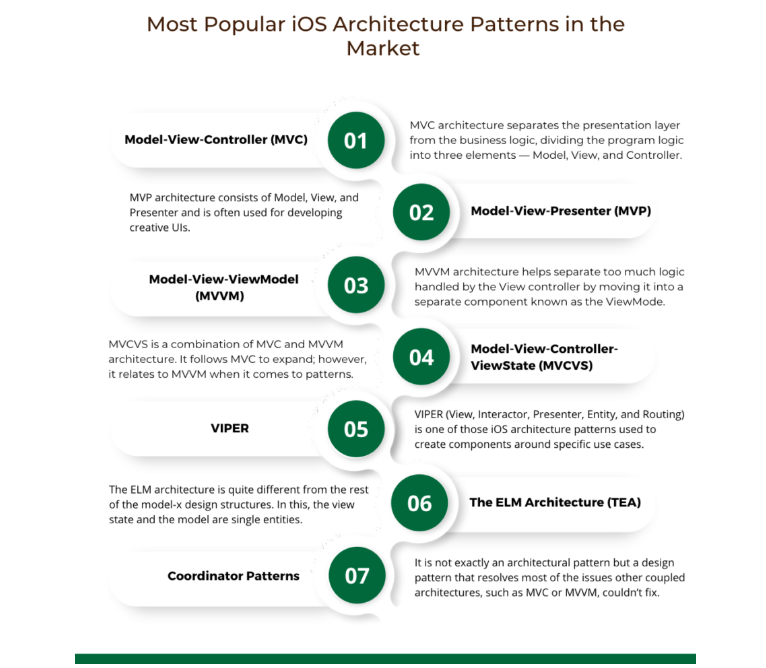
\includegraphics[width=0.8\textwidth]{images/mohinhkientrucios.png}
     \caption{Một số mô hình kiến trúc IOS\cite{MôHinhIOS}.}
    \label{fig:mohinhkientrucios}
\end{figure}
\subsection{Model–View–Controller (MVC)}
\hspace*{0.8cm}Model–View–Controller (MVC) là một trong những mô hình kiến trúc truyền thống được Apple khuyến nghị sử dụng trong phát triển ứng dụng iOS. Mô hình này chia ứng dụng thành ba thành phần chính với vai trò rõ ràng nhằm tăng tính tổ chức và khả năng bảo trì mã nguồn.
  Thành phần đầu tiên, \textbf{Model}, là nơi quản lý dữ liệu và xử lý logic nghiệp vụ. Tiếp theo, \textbf{View} đảm nhiệm việc hiển thị giao diện người dùng và phản hồi các tương tác từ người dùng. Cuối cùng, \textbf{Controller} đóng vai trò trung gian, liên kết giữa Model và View, đồng thời xử lý các logic điều khiển và điều phối luồng dữ liệu.

  Một số ưu điểm nổi bật của mô hình MVC có thể kể đến như: đây là một mẫu kiến trúc phổ biến, không chỉ trong phát triển ứng dụng iOS mà còn cả trong phát triển web; nó cho phép phân tách rõ ràng trách nhiệm giữa các thành phần, đặc biệt là giữa phía máy chủ và máy khách; và nó rất phù hợp với các ứng dụng nhỏ, đơn giản nhờ tính dễ triển khai.

  Tuy nhiên, đi kèm với những lợi ích đó, MVC cũng tồn tại một số hạn chế. Nhược điểm lớn nhất là tình trạng \textit{"Massive View Controller"}, trong đó Controller trở nên quá lớn và phức tạp khi ứng dụng phát triển. Điều này không chỉ làm giảm khả năng kiểm thử mà còn khiến việc bảo trì trở nên khó khăn hơn do sự phụ thuộc chặt chẽ giữa các thành phần trong kiến trúc.

\subsection{Mô hình MVP trong iOS}

\hspace*{0.8cm}Model-View-Presenter (MVP) là một biến thể của mô hình MVC, với mục đích tách biệt rõ ràng hơn giữa phần hiển thị (View) và logic điều khiển (Presenter). Sự phân tách này giúp tăng khả năng kiểm thử và tái sử dụng mã nguồn, đồng thời nâng cao tính linh hoạt trong việc thay đổi và mở rộng ứng dụng. 

  Thành phần của mô hình MVP gồm ba phần chính: \textbf{Model}, giống như trong mô hình MVC, quản lý dữ liệu và xử lý các logic nghiệp vụ; \textbf{View} là giao diện thụ động, chỉ có nhiệm vụ hiển thị dữ liệu và không tham gia vào việc xử lý logic; \textbf{Presenter} là thành phần xử lý toàn bộ logic nghiệp vụ và đảm nhận vai trò cập nhật dữ liệu cho View.

  Một số ưu điểm của mô hình MVP là: \textit{View} hoàn toàn thụ động, dễ dàng kiểm thử và duy trì; việc xác minh chức năng chính xác của từng thành phần trở nên dễ dàng hơn khi chúng được phân tách rõ ràng; \textit{Presenter} có thể được tái sử dụng với nhiều \textit{View} khác nhau, làm cho mã nguồn trở nên linh hoạt và dễ bảo trì.

  Tuy nhiên, mô hình MVP cũng có một số nhược điểm, bao gồm: sự cần thiết phải viết mã \textit{boilerplate} nhiều; \textit{Presenter} có thể trở nên quá lớn và phức tạp khi ứng dụng phát triển; và cuối cùng, MVP không phổ biến bằng mô hình MVVM trong cộng đồng iOS, làm cho việc tìm kiếm tài liệu và hỗ trợ trở nên khó khăn hơn.

\subsection{Mô hình MVVM trong iOS}

\hspace*{0.8cm}MVVM (Model-View-ViewModel) là một mô hình kiến trúc hiện đại được áp dụng rộng rãi trong phát triển ứng dụng iOS, đặc biệt khi kết hợp với các framework reactive như Combine hoặc RxSwift. Mô hình này giúp tách biệt rõ ràng giữa giao diện người dùng và logic nghiệp vụ, tăng khả năng kiểm thử và dễ bảo trì.

  Mô hình MVVM bao gồm ba thành phần chính: \textbf{Model}, giống như trong các mô hình khác, có nhiệm vụ quản lý dữ liệu và logic nghiệp vụ; \textbf{View}, bao gồm các đối tượng \textbf{UIView} và \textbf{UIViewController}, chịu trách nhiệm hiển thị giao diện người dùng; và \textbf{ViewModel}, thành phần chịu trách nhiệm chuẩn bị dữ liệu từ Model và xử lý logic cần thiết để View có thể hiển thị dữ liệu.

  MVVM có bốn nguyên tắc quan trọng cần tuân thủ: \textbf{The Simplicity Principle} (Nguyên tắc đơn giản) yêu cầu mỗi View chỉ nên có một ViewModel và ngược lại; \textbf{The Blendability Principle} (Nguyên tắc hòa trộn) đề xuất ViewModel cần hỗ trợ tối ưu hóa UI; \textbf{The Designability Principle} (Nguyên tắc thiết kế) nhấn mạnh ViewModel phải cung cấp dữ liệu có thể sử dụng tại thời điểm thiết kế; và \textbf{The Testability Principle} (Nguyên tắc kiểm thử) yêu cầu cả Model và ViewModel phải có khả năng kiểm thử độc lập.

  Ưu điểm của mô hình MVVM bao gồm việc tách biệt rõ ràng các thành phần, dễ dàng kiểm thử (đặc biệt là ViewModel), giảm kích thước và trách nhiệm của ViewController, và hỗ trợ binding dữ liệu giữa View và ViewModel. Tuy nhiên, mô hình này cũng có một số nhược điểm, chẳng hạn như sự phức tạp hơn so với MVC, khả năng dẫn đến "Massive ViewModel" nếu không được tổ chức tốt, và yêu cầu cơ chế binding (thủ công hoặc sử dụng thư viện reactive).

  \subsection{MVCVS (Model-View-Controller-ViewState)}

\hspace*{0.8cm}MVCVS là một sự kết hợp giữa hai kiến trúc MVC và MVVM, giúp tách biệt rõ ràng giữa \textbf{Model}, \textbf{View}, \textbf{Controller}, và \textbf{View State}. Trong mô hình này, \textbf{View State} giữ vai trò quan trọng trong việc theo dõi và cập nhật trạng thái giao diện người dùng.

  Ở giai đoạn \textbf{MVCVS Initialization}, View Controller phải tuân theo Model và View State để khởi tạo các thành phần. Khi có bất kỳ thay đổi nào trong \textbf{Model}, \textbf{MVCVS Model Updates} sẽ cập nhật Document Model và View State. Tiếp theo, trong giai đoạn \textbf{MVCVS View Changes}, View State sẽ phân tích Document View Model và View State, từ đó thực hiện các thay đổi đối với View dựa trên các quan sát. \textbf{MVCVS View State} tách biệt View Controller và View State, nơi View State chịu trách nhiệm cập nhật và lắng nghe các thay đổi trong View. Cuối cùng, \textbf{MVCVS Testability} cho phép kiểm tra logic của View Model và Document Model một cách riêng biệt, giúp việc kiểm thử hiệu quả hơn so với mô hình MVC.

  Về ưu điểm, MVCVS mang lại khả năng quản lý hiệu quả cao và dễ dàng kiểm tra các thành phần riêng biệt nhờ các bài kiểm tra tích hợp. Tuy nhiên, nó cũng có nhược điểm là độ phức tạp cao và khó tiếp cận đối với người mới.

  \subsection{VIPER}

\hspace*{0.8cm}VIPER là một mẫu kiến trúc sạch, được sử dụng khi cần tạo các thành phần xoay quanh các trường hợp sử dụng cụ thể trong iOS. VIPER gồm năm thành phần chính: \textbf{View} (giao diện người dùng), \textbf{Interactor} (logic nghiệp vụ), \textbf{Presenter} (điều phối giữa View và Interactor), \textbf{Entity} (mô hình dữ liệu), và \textbf{Routing} (điều hướng giữa các màn hình).

  Ưu điểm của VIPER là dễ quản lý, đặc biệt khi làm việc với nhóm phát triển lớn. Nó giúp tăng khả năng tái sử dụng mã nguồn, kiểm soát UI và giúp dễ dàng kiểm thử mã nhờ vào việc phân tách các thành phần. Hơn nữa, nó giúp giảm thiểu xung đột hợp nhất mã. Tuy nhiên, VIPER có cấu trúc phức tạp đối với ứng dụng nhỏ, yêu cầu thời gian để làm quen và nhiều lớp trung gian có thể ảnh hưởng đến hiệu suất.

  \subsection{The Elm Architecture (TEA)}

\hspace*{0.8cm}TEA là một mô hình kiến trúc đặc biệt trong iOS, khác biệt so với các cấu trúc Model-X truyền thống. Trạng thái giao diện và mô hình được hợp nhất thành một thực thể duy nhất, và mọi cập nhật được gửi đến thực thể này dưới dạng \textbf{messages} và xử lý thông qua \textbf{reducers}. Dòng sự kiện trong TEA được duy trì theo nguyên lý một chiều (unidirectional), tương tự như Flux hoặc Redux.

  Ưu điểm của TEA là khả năng mô tả View như các hàm thuần túy (pure functions) và thực hiện one-way binding từ Model đến View giúp dễ kiểm soát. Tuy nhiên, TEA cũng có nhược điểm, đó là nó tăng độ phức tạp trong các ứng dụng lớn và không phù hợp với mọi loại ứng dụng.

  \subsection{Coordinator Pattern}

\hspace*{0.8cm}Coordinator không phải là một mẫu kiến trúc chính thức mà là một \textbf{design pattern}, giúp giải quyết các vấn đề điều hướng mà MVC hoặc MVVM không xử lý tốt. Coordinator chịu trách nhiệm tạo và giữ tham chiếu đến ViewController hiện tại, đồng thời thực hiện việc điều hướng giữa các màn hình, như việc hiển thị màn hình mới hoặc đẩy ViewController vào Navigation Controller.

  Một trong những ưu điểm lớn của Coordinator là khả năng tách riêng logic điều hướng, giúp mã dễ bảo trì và tăng tính linh hoạt khi chuyển đổi giữa các màn hình. Tuy nhiên, khi triển khai Coordinator, có thể làm tăng độ phức tạp của ứng dụng, yêu cầu thay đổi cách tiếp cận luồng dữ liệu và không cần thiết cho các ứng dụng nhỏ.
\section{Quản lý trạng thái trong ứng dụng iOS}

Quản lý trạng thái hiệu quả là một phần quan trọng trong kiến trúc ứng dụng iOS, đặc biệt khi ứng dụng phát triển về quy mô và độ phức tạp.

\subsection{Các cách tiếp cận quản lý trạng thái}

Quản lý trạng thái có thể được thực hiện qua nhiều phương pháp khác nhau. Dưới đây là ba cách tiếp cận phổ biến:

\paragraph*{1. Quản lý trạng thái cục bộ:}
Trạng thái có thể được lưu trữ trong ViewController thông qua các thuộc tính của nó. Phương pháp này giúp duy trì sự đơn giản trong các ứng dụng nhỏ và dễ dàng quản lý. Một cách để phản ứng với các thay đổi trạng thái là sử dụng \texttt{Property Observers} với \texttt{didSet}, giúp theo dõi và cập nhật khi trạng thái thay đổi.

\paragraph*{2. Reactive Programming:}
Khi cần sự linh hoạt và tính đồng bộ trong quản lý trạng thái, Reactive Programming là một lựa chọn phổ biến. Apple cung cấp framework reactive chính thức của mình là \textbf{Combine Framework}\cite{Combine-Framework}, hỗ trợ quản lý trạng thái và dòng sự kiện một cách dễ dàng. Bên cạnh đó, \textbf{RxSwift} là thư viện reactive phổ biến trong cộng đồng iOS, giúp quản lý trạng thái và sự kiện trong ứng dụng.

\paragraph*{3. Redux-like Architecture:}
Một cách tiếp cận khác là sử dụng kiến trúc giống Redux, trong đó trạng thái được lưu trữ toàn cục trong một \textbf{Store}. Khi có nhu cầu thay đổi trạng thái, các \textbf{Actions} được gửi để mô tả ý định thay đổi. Các \textbf{Reducers} sau đó sẽ xử lý các Action và trả về trạng thái mới, giúp duy trì tính nhất quán và dễ kiểm soát trong việc quản lý trạng thái toàn cục của ứng dụng.


\subsection{State Containers}

\textbf{The Composable Architecture (TCA)} là một framework được phát triển bởi Point-Free, cung cấp cách tiếp cận có nguyên tắc để xây dựng ứng dụng iOS. Framework này giúp tổ chức mã nguồn một cách rõ ràng và dễ kiểm tra.
Cách thức hoạt động của TCA dựa trên bốn thành phần chính:
\paragraph*{1.State:}
State mô tả trạng thái của một tính năng trong ứng dụng. Mỗi tính năng trong TCA sẽ có một State riêng, giúp quản lý và theo dõi trạng thái dễ dàng.
\paragraph*{2.Action:}
Action là các sự kiện có thể xảy ra trong ứng dụng, chúng mô tả những thay đổi có thể xảy ra đối với trạng thái. Mỗi Action có thể dẫn đến việc thay đổi trạng thái của ứng dụng.
\paragraph*{3.Environment:}
Environment là các dependency cần thiết cho logic của tính năng, như các API hoặc các dịch vụ bên ngoài mà ứng dụng cần để hoạt động. Đây là yếu tố giúp logic trở nên dễ kiểm soát và có thể thay đổi khi cần thiết.
\paragraph*{4.Reducer:}
Reducer xử lý logic và cập nhật trạng thái tương ứng khi có Action xảy ra. Nó nhận vào Action và State hiện tại để tính toán và trả về trạng thái mới.


\section{Quản lý phụ thuộc}
Quản lý phụ thuộc (Dependency Injection - DI) là một kỹ thuật quan trọng để tạo ra mã có thể kiểm thử và bảo trì.

\subsection{Các loại Dependency Injection}

Dependency Injection (DI) là một kỹ thuật thiết kế phần mềm giúp tăng tính linh hoạt và khả năng kiểm thử của ứng dụng. DI cho phép các đối tượng cần các phụ thuộc (dependencies) của chúng được cung cấp từ bên ngoài thay vì tự tạo ra. Có ba loại Dependency Injection phổ biến trong lập trình iOS:

\paragraph*{1. Constructor Injection}
Constructor Injection là một phương pháp cung cấp dependencies thông qua một initializer (hàm khởi tạo) của lớp. Các đối tượng cần phụ thuộc sẽ được truyền vào trong quá trình khởi tạo của lớp, giúp đối tượng có thể sử dụng ngay lập tức những dependencies cần thiết mà không cần phải tự tạo chúng. Phương pháp này giúp đảm bảo rằng các đối tượng luôn được khởi tạo với các giá trị hợp lệ và không có tình trạng thiếu dependencies.

Ví dụ về Constructor Injection:

\begin{lstlisting}[language=Swift]
  class NetworkManager {
      private let apiClient: APIClient
  
      init(apiClient: APIClient) {
          self.apiClient = apiClient
      }
  }
  \end{lstlisting}
  
Trong ví dụ này, NetworkManager nhận một đối tượng APIClient thông qua constructor và sử dụng nó để thực hiện các thao tác mạng. Đây là cách tiếp cận mạnh mẽ vì mọi phụ thuộc đều phải được cung cấp trong khi khởi tạo.
\paragraph*{2. Property Injection}
Property Injection là một phương pháp cung cấp dependencies thông qua các thuộc tính của lớp sau khi đối tượng đã được khởi tạo. Thay vì truyền phụ thuộc vào trong initializer, các dependencies sẽ được gán trực tiếp vào các thuộc tính của đối tượng. Phương pháp này mang lại sự linh hoạt trong việc thay đổi hoặc thay thế các dependencies sau khi đối tượng đã được tạo ra.

Ví dụ về Property Injection:
\begin{lstlisting}[language=Swift]
  class NetworkManager {
    var apiClient: APIClient?
}
  \end{lstlisting}
  Ở đây, apiClient có thể được gán giá trị sau khi một đối tượng NetworkManager đã được khởi tạo. Tuy nhiên, phương pháp này có thể gây khó khăn trong việc đảm bảo rằng đối tượng luôn có tất cả các phụ thuộc cần thiết, vì một số phụ thuộc có thể chưa được gán.

\paragraph*{3. Method Injection}
  Method Injection là một phương pháp cung cấp dependencies cho một phương thức cụ thể. Thay vì cung cấp dependencies ở cấp độ lớp như Constructor Injection hay Property Injection, Method Injection cho phép một phương thức nhận vào dependencies mà nó cần trong khi gọi. Phương pháp này rất hữu ích khi chỉ có một số phương thức cụ thể yêu cầu một phụ thuộc đặc biệt mà không cần phải cung cấp nó cho toàn bộ lớp.

  Ví dụ về Method Injection:
  \begin{lstlisting}[language=Swift]
    class DataManager {
        func fetchData(apiClient: APIClient) {
        }
    }
    \end{lstlisting}
    Ở đây, fetchData nhận một đối tượng APIClient làm tham số và sử dụng nó trong quá trình thực hiện yêu cầu mạng. Điều này giúp đảm bảo rằng APIClient chỉ được cung cấp cho các phương thức cần nó, thay vì phải được lưu trữ trong toàn bộ lớp.
\subsection{DI Containers}
    DI Containers (Dependency Injection Containers) giúp quản lý và cung cấp dependencies một cách tự động và có tổ chức. Thay vì phải tạo đối tượng một cách thủ công và tự mình xử lý tất cả các dependencies, DI Containers cho phép bạn khai báo các phụ thuộc và giải quyết chúng một cách tự động, giúp mã nguồn trở nên dễ duy trì và mở rộng hơn. Một số DI Containers phổ biến trong iOS bao gồm:

    \begin{itemize}
      \item \textbf{Swinject:} Swinject là một DI container phổ biến trong cộng đồng iOS, được viết bằng Swift. Nó cung cấp một cách tiếp cận mạnh mẽ để quản lý dependencies trong các ứng dụng iOS, giúp giảm thiểu sự phụ thuộc trực tiếp giữa các lớp. Swinject hỗ trợ tạo đối tượng tự động và cung cấp các dependencies cho các lớp khác khi cần thiết, đồng thời giúp việc kiểm thử và tái sử dụng mã nguồn trở nên dễ dàng hơn.

      \textbf{Ví dụ về Swinject:}
      \begin{lstlisting}[language=Swift]
        import Swinject

        class NetworkManager {
            func fetchData() {
                print("Fetching data from the network...")
            }
        }

        class ViewController {
            private let networkManager: NetworkManager

            init(networkManager: NetworkManager) {
                self.networkManager = networkManager
            }

            func startFetchingData() {
                networkManager.fetchData()
            }
        }

    let container = Container()
    container.register(NetworkManager.self) { _ in NetworkManager() }
    container.register(ViewController.self) { r in
    ViewController(networkManager: r.resolve(NetworkManager.self)!)
        }

    let viewController = container.resolve(ViewController.self)!
        viewController.startFetchingData()
      \end{lstlisting}
      Trong ví dụ trên, Swinject giúp chúng ta dễ dàng đăng ký và giải quyết dependencies. Container quản lý các đối tượng và tự động cung cấp chúng khi yêu cầu.

      \item \textbf{Service Locator:} Service Locator là một giải pháp thay thế cho Dependency Injection. Thay vì truyền dependencies qua constructor hoặc các phương thức, Service Locator cung cấp một trung tâm quản lý các dịch vụ, nơi các lớp có thể yêu cầu các dịch vụ khi cần. Mặc dù phương pháp này giảm thiểu sự cần thiết phải truyền dependencies, nhưng nó có thể dẫn đến mã nguồn khó kiểm soát hơn khi số lượng dependencies tăng lên. Do đó, mặc dù Service Locator là một giải pháp đơn giản và dễ triển khai, nhưng nó có thể gây khó khăn trong việc theo dõi sự thay đổi của các dependencies trong ứng dụng lớn.

      \textbf{Ví dụ về Service Locator:}
      \begin{lstlisting}[language=Swift]
        class NetworkManager {
            func fetchData() {
                print("Fetching data from the network...")
            }
        }

        class ServiceLocator {
            static var shared = ServiceLocator()
            private var services = [String: Any]()

            func register<T>(_ service: T) {
                let key = String(describing: T.self)
                services[key] = service
            }

            func resolve<T>() -> T? {
                let key = String(describing: T.self)
                return services[key] as? T
            }
        }


        let networkManager = NetworkManager()
        ServiceLocator.shared.register(networkManager)

        let retrievedNetworkManager = ServiceLocator.shared.resolve() as NetworkManager?
        retrievedNetworkManager?.fetchData()
      \end{lstlisting}
      Trong ví dụ này, Service Locator chịu trách nhiệm quản lý và cung cấp đối tượng `NetworkManager` khi cần thiết. Mặc dù đơn giản, nhưng cách tiếp cận này có thể gây khó khăn trong việc duy trì mã nguồn khi có nhiều dependencies.
    \end{itemize}
    
\section{Cách thiết kế giao diện người dùng}
iOS cung cấp hai framework chính để xây dựng giao diện người dùng: \textbf{UIKit} và \textbf{SwiftUI}.

\subsection{UIKit}
UIKit là framework UI truyền thống cho iOS, sử dụng mô hình lập trình mệnh lệnh và dựa trên lớp:
\begin{itemize}
  \item \textbf{Auto Layout:} Giúp tạo UI thích ứng với các kích thước màn hình khác nhau.
  \item \textbf{View Controller Lifecycle:} Hiểu rõ vòng đời của \textbf{UIViewController} là chìa khóa để quản lý tài nguyên và trạng thái.
  \item \textbf{Reusable Views:} Tái sử dụng views để cải thiện hiệu suất vào khả năng bảo trì.
\end{itemize}

\subsection{SwiftUI}
SwiftUI là framework UI khai báo mới của Apple, giới thiệu từ iOS 13.
\begin{itemize}
  \item \textbf{View Basics:} Sử dụng cấu trúc \texttt{protocol View} để xây dựng UI.
  \item \textbf{State và Binding:} Sử dụng \texttt{property wrappers} để quản lý trạng thái.
  \item \textbf{ObservableObject và EnvironmentObject:} Cung cấp các cơ chế để quản lý trạng thái phức tạp.
\end{itemize}

\subsection{So sánh UIKit và SwiftUI}

\begin{center}
\begin{tabular}{|l|l|l|}
\hline
\textbf{Khía cạnh} & \textbf{UIKit} & \textbf{SwiftUI} \\
\hline
Năm ra mắt & 2008 & 2019 \\
\hline
Loại lập trình & Mệnh lệnh & Khai báo \\
\hline
Cấu trúc & Dựa trên lớp (Class-based) & Dựa trên struct (Struct-based) \\
\hline
Trạng thái & Tự quản lý & Property wrappers \\
\hline
Hỗ trợ iOS & iOS 2+ & iOS 13+ \\
\hline
Độ ổn định & Rất ổn định & Đang phát triển \\
\hline
Học tập & Phức tạp & Dễ dàng hơn \\
\hline
Tùy biến & Rất linh hoạt & Hạn chế hơn \\
\hline
\end{tabular}
\end{center}

\section{Xử lý Dữ liệu}

Quản lý dữ liệu là một phần quan trọng trong phát triển ứng dụng iOS. Apple cung cấp nhiều giải pháp khác nhau để lưu trữ và truy xuất dữ liệu, phù hợp với các mục đích và quy mô sử dụng khác nhau. Dưới đây là so sánh và mô tả chi tiết các giải pháp lưu trữ dữ liệu phổ biến trong hệ sinh thái iOS.


\subsection{Core Data}
Core Data\cite{Core-Data} là một framework của Apple được thiết kế để quản lý graph đối tượng và vòng đời dữ liệu trong ứng dụng iOS, không phải là một cơ sở dữ liệu thuần túy. Nó cung cấp một cách tiếp cận mạnh mẽ để làm việc với dữ liệu có cấu trúc phức tạp và lưu trữ trong các ứng dụng iOS.

\textbf{Kiến trúc Core Data} bao gồm một số thành phần quan trọng. Đầu tiên là \textbf{NSManagedObjectModel}, mô tả cấu trúc của các entities, attributes và relationships trong ứng dụng. \textbf{NSManagedObjectContext} là không gian làm việc để thực hiện các thao tác CRUD (Create, Read, Update, Delete), trong khi \textbf{NSPersistentStoreCoordinator} điều phối giữa object model và persistent store. Đối với các ứng dụng từ iOS 10 trở lên, \textbf{NSPersistentContainer} cung cấp một cách dễ dàng để đóng gói toàn bộ stack Core Data, giúp đơn giản hóa việc cấu hình và quản lý dữ liệu. Để truy vấn dữ liệu, \textbf{NSFetchRequest} được sử dụng để lấy dữ liệu từ persistent store.

Core Data cung cấp một số \textbf{đặc điểm chính}, bao gồm khả năng quản lý object graph và các mối quan hệ phức tạp, lưu trữ dữ liệu thông qua SQLite backend, và hỗ trợ tính năng tải dữ liệu một cách lười biếng (lazy loading). Hệ thống còn tích hợp kiểm tra dữ liệu và hỗ trợ migration/versioning, giúp dễ dàng cập nhật và bảo trì dữ liệu qua các phiên bản ứng dụng khác nhau.

Về \textbf{ưu điểm}, Core Data tích hợp chặt chẽ với hệ sinh thái của Apple, bao gồm các công cụ thiết kế mô hình dữ liệu trực quan. Nó còn hỗ trợ đồng bộ hóa dữ liệu với CloudKit và có khả năng quản lý bộ nhớ thông minh, tối ưu hóa việc sử dụng tài nguyên.
Tuy nhiên, Core Data cũng có \textbf{nhược điểm}. Đường cong học tập của nó khá dốc, khiến người mới làm quen cảm thấy khó khăn trong việc sử dụng. Việc debug cũng trở nên phức tạp và khó khăn, và Core Data không hoàn toàn thread-safe, điều này có thể gây ra các vấn đề khi thao tác với dữ liệu từ nhiều luồng cùng lúc.

Cuối cùng, \textbf{Core Data} là sự lựa chọn lý tưởng cho các ứng dụng có dữ liệu phức tạp và nhiều quan hệ. Nó cũng rất phù hợp cho các dự án dài hạn cần bảo trì tốt và dễ dàng cập nhật dữ liệu trong suốt vòng đời phát triển.

\subsection{Realm}
Realm là một cơ sở dữ liệu di động mã nguồn mở được thiết kế để thay thế Core Data với hiệu suất cao và API đơn giản, giúp các nhà phát triển dễ dàng xây dựng ứng dụng với dữ liệu lưu trữ hiệu quả. Đặc biệt, Realm cung cấp một số tính năng nổi bật, làm cho nó trở thành một lựa chọn hấp dẫn trong việc quản lý dữ liệu cho các ứng dụng di động.

\textbf{Đặc điểm chính} của Realm bao gồm khả năng hoạt động đa nền tảng, hỗ trợ cả iOS và Android, giúp các nhà phát triển xây dựng ứng dụng cross-platform dễ dàng hơn. Một tính năng quan trọng khác của Realm là kiến trúc "zero-copy", cho phép truy cập dữ liệu trực tiếp mà không cần sao chép bộ nhớ, mang lại hiệu suất cao. Realm cũng hỗ trợ lập trình reactive, giúp đơn giản hóa việc xử lý các thay đổi dữ liệu và cập nhật UI trong ứng dụng. Một điểm mạnh khác của Realm là tính năng thread-safe theo từng instance của Realm, đảm bảo dữ liệu an toàn khi truy cập từ nhiều luồng khác nhau. Nó còn hỗ trợ mã hóa và đồng bộ hóa dữ liệu thời gian thực, mang lại sự linh hoạt cho các ứng dụng yêu cầu tính năng đồng bộ cao.

\textbf{Ưu điểm} của Realm là API đơn giản và dễ học, giúp tiết kiệm thời gian cho các nhà phát triển khi tích hợp vào ứng dụng. Ngoài ra, hiệu suất của Realm rất cao, điều này rất quan trọng đối với các ứng dụng cần xử lý lượng dữ liệu lớn. Realm còn hỗ trợ đồng bộ hóa dữ liệu theo thời gian thực, một tính năng cần thiết trong các ứng dụng cần cập nhật dữ liệu liên tục. Tài liệu của Realm rất rõ ràng và dễ tiếp cận, cùng với cộng đồng lớn và nhiệt tình hỗ trợ, giúp nhà phát triển giải quyết các vấn đề nhanh chóng.
Mặc dù có nhiều ưu điểm, \textbf{Realm} cũng có \textbf{nhược điểm}. Đầu tiên, Realm không tích hợp sâu với iOS, điều này có thể gây khó khăn khi tích hợp với các framework khác của Apple. Thứ hai, Realm không hỗ trợ struct, thay vào đó yêu cầu sử dụng class kế thừa từ \texttt{Object}, điều này có thể gây ra một số bất tiện cho các nhà phát triển. Thêm vào đó, một số giới hạn trong model threading và truy vấn phức tạp có thể ảnh hưởng đến tính linh hoạt của ứng dụng khi xử lý các tình huống dữ liệu phức tạp.

Về \textbf{khi nên dùng}, Realm là sự lựa chọn tuyệt vời cho các ứng dụng cross-platform, giúp dễ dàng triển khai trên cả iOS và Android mà không gặp phải vấn đề tương thích. Nó cũng rất thích hợp cho các dự án yêu cầu hiệu suất cao và đồng bộ hóa dữ liệu theo thời gian thực, ví dụ như các ứng dụng cần tính năng đồng bộ dữ liệu giữa các thiết bị. Cuối cùng, Realm rất phù hợp cho các dự án ưu tiên offline-first, khi ứng dụng cần có khả năng hoạt động tốt mà không phụ thuộc quá nhiều vào kết nối mạng.

\subsection{SQLite}
SQLite là một hệ quản trị cơ sở dữ liệu quan hệ nhỏ gọn, không yêu cầu server và được sử dụng rộng rãi trên thế giới nhờ vào sự đơn giản, hiệu quả và dễ triển khai. Với thiết kế "self-contained", SQLite không cần cài đặt riêng biệt hoặc máy chủ, khiến nó trở thành một lựa chọn phổ biến cho các ứng dụng di động và ứng dụng nhúng.

\textbf{Đặc điểm chính} của SQLite là tính tự chứa và không yêu cầu cấu hình, giúp dễ dàng tích hợp vào các ứng dụng mà không gặp phải những phức tạp của việc cài đặt và cấu hình server. SQLite rất nhẹ và đáng tin cậy, đồng thời hỗ trợ đa nền tảng (cross-platform), có thể chạy trên nhiều hệ điều hành khác nhau. SQLite hỗ trợ đầy đủ SQL, cho phép thực hiện các thao tác truy vấn cơ sở dữ liệu mạnh mẽ và linh hoạt. Hệ thống này tuân thủ chuẩn ACID, đảm bảo các thao tác dữ liệu được thực hiện một cách an toàn và chính xác, ngay cả khi hệ thống gặp sự cố.

\textbf{Ưu điểm} của SQLite là khả năng kiểm soát toàn diện schema và truy vấn. Điều này có nghĩa là bạn có thể hoàn toàn tùy chỉnh cấu trúc dữ liệu và các câu truy vấn theo nhu cầu của ứng dụng. SQLite cũng rất phù hợp với các truy vấn phức tạp nhờ vào tính mạnh mẽ của SQL. Ngoài ra, SQLite rất dễ dàng để sao lưu và khôi phục, một yếu tố quan trọng trong việc bảo vệ dữ liệu của ứng dụng.

Tuy nhiên, \textbf{SQLite} cũng có \textbf{nhược điểm}. Một trong những khó khăn là bạn phải tự xử lý các vấn đề về thread-safe và migration, vì SQLite không cung cấp các công cụ tự động hóa cho những vấn đề này. SQLite cũng không hỗ trợ object mapping tự động, điều này có thể khiến việc làm việc với các đối tượng trong ứng dụng trở nên phức tạp hơn. Cuối cùng, SQLite không phải là công cụ lý tưởng cho các ứng dụng sử dụng mô hình lập trình reactive, vì nó không hỗ trợ cập nhật dữ liệu theo thời gian thực một cách tự động.

Về \textbf{khi nên dùng}, SQLite là lựa chọn lý tưởng nếu bạn cần kiểm soát hoàn toàn cơ sở dữ liệu và muốn thực hiện các thao tác SQL phức tạp. Nó cũng phù hợp với các ứng dụng không yêu cầu tích hợp chặt với hệ sinh thái iOS, ví dụ như các ứng dụng nhỏ hoặc nhúng, nơi cần sự đơn giản và hiệu suất cao.

\subsection{UserDefaults}
\textbf{Định nghĩa:} \texttt{UserDefaults} là một hệ thống lưu trữ key-value đơn giản, được thiết kế để lưu trữ dữ liệu nhỏ và không nhạy cảm. Đây là công cụ lý tưởng cho việc lưu trữ các cài đặt hoặc trạng thái người dùng trong ứng dụng iOS.

\textbf{Đặc điểm chính:} \texttt{UserDefaults} hỗ trợ lưu trữ dữ liệu dưới dạng key-value. Với API đơn giản, nó cho phép lưu trữ các kiểu cơ bản như String, Int, Bool, Date, và các đối tượng đơn giản khác. Hệ thống này tự động đồng bộ hóa và có cache nội bộ, đồng thời có khả năng đồng bộ với iCloud, cho phép dữ liệu người dùng được lưu trữ và truy cập trên nhiều thiết bị Apple.

\textbf{Ưu điểm:} Với \texttt{UserDefaults}, việc lưu trữ dữ liệu trở nên dễ dàng và hiệu quả. Nó có hiệu suất cao khi lưu trữ các dữ liệu nhỏ và không yêu cầu cấu hình phức tạp. \texttt{UserDefaults} rất thích hợp để lưu trữ trạng thái người dùng hoặc các cài đặt của ứng dụng.

\textbf{Nhược điểm:} Mặc dù dễ sử dụng, \texttt{UserDefaults} không phù hợp cho việc lưu trữ dữ liệu lớn hoặc nhạy cảm vì thiếu các tính năng bảo mật. Thêm vào đó, nó không hỗ trợ các thao tác phức tạp như lọc, truy vấn, hoặc giao dịch dữ liệu, điều này có thể hạn chế trong các ứng dụng cần thao tác với dữ liệu phức tạp.

\textbf{Khi nên dùng:} \texttt{UserDefaults} là lựa chọn lý tưởng khi bạn cần lưu trữ các thông tin đơn giản như theme, ngôn ngữ, âm thanh, hoặc đánh dấu các trạng thái hoàn thành, như đã hoàn thành hướng dẫn sử dụng. Nó cũng rất phù hợp cho việc lưu các cấu hình đơn giản hoặc flags trong ứng dụng.

\subsection{Keychain}
\textbf{Định nghĩa:} \texttt{Keychain} là hệ thống lưu trữ an toàn được thiết kế để bảo vệ thông tin nhạy cảm như mật khẩu, token xác thực và các dữ liệu quan trọng khác. Hệ thống này đảm bảo rằng dữ liệu được mã hóa và chỉ có thể truy cập thông qua các phương thức bảo mật.

\textbf{Đặc điểm chính:} \texttt{Keychain} lưu trữ dữ liệu với mã hóa mạnh mẽ, giúp bảo vệ thông tin nhạy cảm khỏi các mối đe dọa bên ngoài. Dữ liệu trong \texttt{Keychain} tồn tại lâu dài, ngay cả khi ứng dụng bị xóa. Nó hỗ trợ xác thực sinh trắc học như Face ID và Touch ID, đồng thời có thể chia sẻ giữa các ứng dụng của cùng một nhà phát triển. \texttt{Keychain} cũng hỗ trợ đồng bộ hóa với iCloud, cho phép người dùng truy cập dữ liệu bảo mật trên nhiều thiết bị Apple.

\textbf{Ưu điểm:} Một trong những ưu điểm chính của \texttt{Keychain} là mức độ bảo mật cao, làm cho nó trở thành lựa chọn lý tưởng cho việc lưu trữ các thông tin nhạy cảm. Hệ thống này hỗ trợ xác thực bằng Face ID và Touch ID, cung cấp một lớp bảo vệ thêm cho dữ liệu. Hơn nữa, dữ liệu trong \texttt{Keychain} tồn tại lâu dài và có thể được sử dụng trên nhiều thiết bị.

\textbf{Nhược điểm:} Tuy nhiên, \texttt{Keychain} cũng có một số hạn chế. API của nó phức tạp và khó sử dụng hơn so với các giải pháp lưu trữ thông thường, đòi hỏi người phát triển phải có kiến thức chuyên sâu. Thêm vào đó, việc truy cập và thao tác dữ liệu trong \texttt{Keychain} thường chậm hơn so với lưu trữ thông thường. Cuối cùng, việc debug và kiểm tra dữ liệu trong \texttt{Keychain} cũng gặp khó khăn do tính bảo mật cao.

\textbf{Khi nên dùng:} \texttt{Keychain} là giải pháp lý tưởng khi bạn cần lưu trữ các thông tin nhạy cảm như mật khẩu, token xác thực, hoặc các thông tin bảo mật khác. Nó rất phù hợp cho những ứng dụng có yêu cầu bảo mật cao, nơi mà việc đảm bảo an toàn dữ liệu người dùng là ưu tiên hàng đầu.
\section{Xử lý bất đồng bộ}

Xử lý tác vụ bất đồng bộ là một phần thiết yếu trong kiến trúc ứng dụng iOS hiện đại, giúp đảm bảo giao diện người dùng mượt mà và phản hồi tốt. Swift cung cấp nhiều phương pháp để xử lý bất đồng bộ, từ truyền thống đến hiện đại, mỗi phương pháp có ưu và nhược điểm riêng phù hợp với từng hoàn cảnh.

\subsection{Completion Handlers}
\textbf{Định nghĩa:} Completion handlers là cơ chế truyền thống trong iOS để xử lý các tác vụ bất đồng bộ, trong đó closures được sử dụng để thông báo khi một tác vụ hoàn thành. Khi hàm bất đồng bộ hoàn thành, closure sẽ được gọi để tiếp tục xử lý.

\textbf{Cơ chế hoạt động:} Một hàm bất đồng bộ trong iOS sẽ nhận một closure làm tham số. Closure này được gọi khi tác vụ bất đồng bộ kết thúc, cho phép người phát triển thực hiện các hành động tiếp theo. Thường thì, kiểu dữ liệu \texttt{Result} được sử dụng để phân biệt giữa thành công và thất bại của tác vụ, giúp việc xử lý lỗi và kết quả trở nên rõ ràng hơn.

\textbf{Ưu điểm:} Completion handlers rất dễ hiểu và sử dụng rộng rãi trong cộng đồng lập trình iOS. Không cần phải cài đặt thêm thư viện bên ngoài, việc sử dụng closure giúp tiết kiệm thời gian và đơn giản hóa mã nguồn. Ngoài ra, completion handlers tương thích với tất cả các phiên bản iOS, không yêu cầu tính năng đặc biệt.

\textbf{Nhược điểm:} Tuy nhiên, việc sử dụng completion handlers cũng gặp phải một số vấn đề. Khi chuỗi nhiều tác vụ bất đồng bộ được gọi, rất dễ rơi vào tình trạng \textit{callback hell}, nơi mã trở nên khó hiểu và khó bảo trì. Thêm vào đó, việc truyền lỗi giữa các callback có thể gặp khó khăn, và nếu không cẩn thận, việc quên gọi completion handler có thể gây lỗi trong ứng dụng. Hơn nữa, khi cần thực hiện các tác vụ song song hoặc tuần tự một cách tối ưu, completion handlers có thể không phải là giải pháp hiệu quả nhất.

\subsection{Promises}
\textbf{Định nghĩa:} Promises là một mô hình xử lý bất đồng bộ dựa trên hướng đối tượng, giúp các tác vụ bất đồng bộ được thực hiện tuần tự và dễ dàng quản lý. Mô hình này thường được sử dụng thông qua các thư viện như \texttt{PromiseKit} trong iOS, và nó cung cấp một cách tiếp cận rõ ràng hơn so với completion handlers truyền thống.

\textbf{Cơ chế hoạt động:} Một \texttt{Promise} đại diện cho kết quả sẽ có trong tương lai, giúp mã nguồn dễ hiểu hơn khi xử lý bất đồng bộ. Để xử lý kết quả, ta sử dụng \texttt{.then}, cho phép tiếp tục chuỗi các tác vụ bất đồng bộ. Khi có lỗi xảy ra, \texttt{.catch} sẽ giúp xử lý lỗi một cách tập trung, thay vì phải làm điều này ở nhiều nơi trong mã nguồn. Mô hình Promise cũng dễ dàng kết hợp và biến đổi, giúp việc quản lý các tác vụ bất đồng bộ trở nên thuận tiện và linh hoạt hơn.

\textbf{Ưu điểm:} Promises cung cấp cú pháp rõ ràng và dễ hiểu, đặc biệt là giúp tránh tình trạng \textit{callback hell} khi chuỗi các tác vụ trở nên dài và phức tạp. Chúng hỗ trợ thực hiện các tác vụ song song hoặc tuần tự một cách dễ dàng và hiệu quả, đồng thời quản lý lỗi tập trung, giúp mã nguồn trở nên gọn gàng hơn. Hơn nữa, Promises hỗ trợ chaining (nối tiếp các tác vụ) và transform (biến đổi) dữ liệu, cho phép tạo ra các chuỗi bất đồng bộ phức tạp một cách mượt mà.

\textbf{Nhược điểm:} Tuy nhiên, Promises yêu cầu cài đặt các thư viện bên thứ ba như \texttt{PromiseKit}, điều này có thể làm tăng độ phức tạp của dự án ban đầu. Ngoài ra, mặc dù Promises giúp đơn giản hóa mã nguồn về lâu dài, nhưng người lập trình có thể cần thời gian để làm quen với mô hình này. Cuối cùng, việc debug mã sử dụng Promises có thể khó khăn hơn so với mã đồng bộ truyền thống, do các kết quả và lỗi được xử lý sau khi tác vụ hoàn thành.
\subsection{Async/Await}
\textbf{Định nghĩa:} Từ iOS 15 trở đi, Swift hỗ trợ cú pháp \texttt{async/await}, một mô hình mới cho phép viết mã bất đồng bộ theo cách dễ đọc và dễ quản lý hơn, giống như code đồng bộ truyền thống. Với \texttt{async/await}, mã bất đồng bộ không còn cần đến các callback hoặc closure phức tạp, giúp cải thiện khả năng duy trì và mở rộng ứng dụng.

\textbf{Cơ chế hoạt động:} Cú pháp \texttt{async} được sử dụng để đánh dấu một hàm là bất đồng bộ, trong khi \texttt{await} giúp tạm dừng thực thi của hàm cho đến khi có kết quả trả về. Điều này cho phép viết mã theo kiểu tuần tự mà không bị chặn lại bởi các tác vụ bất đồng bộ. Swift cũng hỗ trợ cấu trúc concurrency rõ ràng thông qua \texttt{Task} và \texttt{TaskGroup}, giúp dễ dàng quản lý và tổ chức các tác vụ đồng thời. Mô hình này cũng dễ dàng kết hợp với \texttt{try-catch} để xử lý lỗi, giúp mã nguồn trở nên mượt mà và dễ đọc hơn.

\textbf{Ưu điểm:} Cú pháp \texttt{async/await} giúp mã nguồn trở nên gọn gàng, dễ đọc và dễ duy trì, đặc biệt khi so với các mô hình callback truyền thống. Quản lý luồng logic và xử lý lỗi trở nên tự nhiên và trực quan hơn, do không cần phải lồng nhiều closure vào nhau. Hơn nữa, cú pháp này tích hợp sâu vào hệ sinh thái của Apple, từ iOS, macOS đến các dịch vụ như CloudKit và URLSession, giúp lập trình viên dễ dàng tiếp cận và sử dụng.

\textbf{Nhược điểm:} Một nhược điểm lớn của cú pháp \texttt{async/await} là yêu cầu phiên bản iOS 15 trở lên, điều này có thể gây khó khăn khi phát triển ứng dụng cần hỗ trợ các phiên bản cũ hơn. Thêm vào đó, để tận dụng được lợi ích của \texttt{async/await}, có thể cần phải refactor lại call stack của các hàm, điều này có thể mất thời gian. Cuối cùng, nếu không quản lý cẩn thận việc hủy các tác vụ bằng \texttt{Task.cancel()}, có thể gây ra vấn đề rò rỉ bộ nhớ.
\subsection{Combine Framework}
\textbf{Định nghĩa:} Combine là một framework lập trình reactive được Apple phát triển, ra mắt từ iOS 13, nhằm hỗ trợ xử lý bất đồng bộ dựa trên dữ liệu và sự kiện. Combine cung cấp một cách tiếp cận hiệu quả để xử lý các luồng dữ liệu và sự kiện trong ứng dụng, giúp lập trình viên có thể dễ dàng quản lý và biến đổi dữ liệu theo cách thức phản ứng với các thay đổi.

\textbf{Cơ chế hoạt động:} Combine dựa trên mô hình \textit{Publisher/Subscriber}, trong đó \texttt{Publisher} phát ra giá trị, và \texttt{Subscriber} nhận và xử lý những giá trị này. Lập trình viên có thể tạo ra các chuỗi pipeline để xử lý và biến đổi dữ liệu, bao gồm việc lọc, kết hợp, hoặc áp dụng các phép toán phức tạp lên dữ liệu. Framework này hỗ trợ việc quản lý backpressure, giúp đảm bảo rằng hệ thống không bị quá tải bởi các sự kiện đến quá nhanh. Combine kết hợp mạnh mẽ với \texttt{SwiftUI}, cho phép xây dựng giao diện người dùng động và phản ứng với các thay đổi trong dữ liệu.

\textbf{Ưu điểm:} Một trong những ưu điểm lớn của Combine là khả năng tích hợp chặt chẽ với Swift và toàn bộ hệ sinh thái Apple, làm cho việc xây dựng ứng dụng trở nên liền mạch và hiệu quả. Framework cung cấp hàng trăm operators hỗ trợ biến đổi và lọc dữ liệu, giúp lập trình viên có thể thực hiện các tác vụ phức tạp một cách dễ dàng. Ngoài ra, Combine tự động quản lý bộ nhớ thông qua \texttt{AnyCancellable}, giúp giảm bớt nỗi lo về việc giải phóng tài nguyên. Combine cho phép xử lý đồng bộ và bất đồng bộ một cách nhất quán, giúp quản lý dữ liệu và sự kiện một cách hiệu quả.

\textbf{Nhược điểm:} Một nhược điểm của Combine là learning curve khá cao, yêu cầu lập trình viên phải hiểu rõ về lập trình reactive và các khái niệm liên quan. Thêm vào đó, Combine yêu cầu iOS 13 trở lên, điều này có thể hạn chế việc sử dụng trong các ứng dụng cần hỗ trợ các phiên bản iOS cũ hơn. Việc debugging các pipeline phức tạp cũng có thể gặp khó khăn, đặc biệt khi chuỗi các phép toán trở nên dài và khó theo dõi. Cuối cùng, mặc dù Combine mạnh mẽ, nhưng nó không hỗ trợ đa nền tảng như \texttt{RxSwift}, điều này có thể là một hạn chế nếu bạn muốn phát triển ứng dụng trên nhiều nền tảng.
\section{Kết luận}

Trong kiến trúc ứng dụng iOS hiện đại, không chỉ có sự phân tách rõ ràng giữa các tầng chức năng như UI, Business Logic và Data, mà còn chú trọng đến khả năng mở rộng, dễ bảo trì và hiệu suất của ứng dụng. Mục tiêu này đạt được thông qua việc áp dụng các mô hình kiến trúc như MVC, MVVM, VIPER, kết hợp với các kỹ thuật xử lý bất đồng bộ hiện đại như \texttt{Completion Handlers}, \texttt{Promises}, \texttt{Async/Await}, và \texttt{Combine}. Những kỹ thuật này giúp xây dựng ứng dụng mượt mà, linh hoạt và thân thiện với người dùng.

\vspace{0.5em}

Mỗi cách tiếp cận này đều có những ưu và nhược điểm riêng, vì vậy, việc lựa chọn phương pháp phù hợp cần dựa trên yêu cầu của dự án và phiên bản iOS mà ứng dụng hỗ trợ. Cụ thể:

\begin{itemize}
\item \textbf{Completion Handlers} vẫn là lựa chọn đơn giản và phổ biến, nhờ vào tính linh hoạt và dễ hiểu.
\item \textbf{Promises} mang lại cú pháp rõ ràng hơn cho các chuỗi bất đồng bộ, giúp mã nguồn dễ theo dõi và bảo trì.
\item \textbf{Async/Await} đang dần trở thành tiêu chuẩn mới nhờ vào sự rõ ràng và tích hợp sâu trong ngôn ngữ Swift, đồng thời cải thiện khả năng đọc hiểu mã nguồn.
\item \textbf{Combine} mở ra hướng lập trình phản ứng hiện đại, đặc biệt phù hợp với các ứng dụng yêu cầu nhiều tương tác và dữ liệu động.
\end{itemize}

Việc lựa chọn kiến trúc và công nghệ phù hợp không chỉ giúp tối ưu hóa hiệu suất mà còn tạo ra trải nghiệm người dùng vượt trội. Trong bối cảnh hệ sinh thái Apple không ngừng phát triển, việc nắm vững và ứng dụng linh hoạt các kỹ thuật hiện đại sẽ là chìa khóa giúp các nhà phát triển iOS tạo ra những sản phẩm thành công và bền vững.



